\documentclass[10pt]{article}

\usepackage[margin=.76in]{geometry}
\usepackage[T1]{fontenc}
\usepackage{libertinus}
\usepackage{microtype}
\usepackage{mathtools,amssymb,amsthm}
\usepackage{booktabs}
\usepackage{enumitem}
\usepackage{titlesec}
\usepackage{fancyhdr}
\usepackage{xcolor}
\usepackage{tikz}
\usetikzlibrary{arrows.meta,positioning}
\usepackage[hidelinks]{hyperref}
\usepackage{orcidlink}

\definecolor{ink}{HTML}{263238}
\definecolor{blue}{HTML}{356A8A}
\definecolor{gold}{HTML}{C28A35}
\definecolor{pale}{HTML}{EDF3F6}
\colorlet{orcidlogocol}{black}
\hypersetup{
  pdftitle={Behavioral Embeddings and Propensity Neighborhoods for Program Recommendation},
  pdfauthor={J. R. Landers},
  pdfsubject={Accessible treatment of behavioral embeddings, propensity neighborhoods, calibration, and program recommendation},
  pdfkeywords={recommender systems, energy programs, propensity models, behavioral embeddings, customer neighborhoods, calibration}
}

\setlength{\parindent}{1em}
\setlength{\parskip}{0pt}
\linespread{0.96}
\setlength{\abovedisplayskip}{3.5pt plus 1pt minus 1pt}
\setlength{\belowdisplayskip}{3.5pt plus 1pt minus 1pt}
\setlength{\textfloatsep}{5pt plus 2pt minus 2pt}
\setlength{\floatsep}{4pt plus 2pt minus 2pt}
\setlist{nosep,leftmargin=1.35em}
\setcounter{secnumdepth}{2}
\titleformat{\section}{\large\bfseries\scshape}{\thesection}{0.6em}{}
\titleformat{\subsection}{\normalsize\bfseries}{\thesubsection}{0.55em}{}
\titlespacing*{\section}{0pt}{.75ex plus .2ex}{.3ex}
\titlespacing*{\subsection}{0pt}{.6ex plus .2ex}{.2ex}

\newtheoremstyle{noteplain}{.35ex}{.35ex}{\itshape}{}{\bfseries}{.}{.4em}{}
\theoremstyle{noteplain}
\newtheorem{theorem}{Theorem}
\newtheorem{proposition}[theorem]{Proposition}
\newtheorem{corollary}[theorem]{Corollary}
\theoremstyle{definition}
\newtheorem{remark}[theorem]{Remark}

\makeatletter
\renewenvironment{proof}[1][\proofname]{\par
  \pushQED{\qed}%
  \normalfont \topsep4\p@\@plus4\p@\relax
  \trivlist
  \item[\hskip\labelsep\bfseries #1\@addpunct{.}]\ignorespaces
}{\popQED\endtrivlist\@endpefalse}
\makeatother

\newcommand{\E}{\mathbb E}
\newcommand{\cA}{\mathcal A}
\newcommand{\cN}{\mathcal N}
\newcommand{\argmax}{\operatorname*{arg\,max}}
\newcommand{\argmin}{\operatorname*{arg\,min}}

\pagestyle{fancy}
\fancyhf{}
\fancyhead[L]{\footnotesize\scshape Propensity Neighborhoods}
\fancyhead[R]{\footnotesize J. R. Landers}
\fancyfoot[C]{\footnotesize\thepage}
\renewcommand{\headrulewidth}{0.35pt}
\setlength{\headheight}{13pt}

\begin{document}

\begin{center}
  {\LARGE\bfseries Behavioral Embeddings and Propensity Neighborhoods for Program Recommendation\par}
  \vspace{0.55em}
  {\large J. R. Landers\,\orcidlink{0000-0003-1872-6179}\par}
  \vspace{0.08em}
  {\small September 2026}
\end{center}

\section{The problem and the idea}

A utility often has several programs that a customer could join. A propensity model can score each eligible program and recommend the one with the largest predicted enrollment probability. This is a sensible baseline, but it can miss local patterns: the model may repeatedly overpredict or underpredict a program for customers with similar behavior.

We study a simple response. First, compress each customer's behavioral history into an embedding. Second, estimate a propensity for every program. Third, find historical customers who look like the target customer and use their out-of-fold prediction errors to make a local correction. The central difficulty is that a more detailed match leaves fewer peers. A useful recommender must balance similarity against support.

The evidence gives a clear division of labor. Behavioral embeddings provide the main predictive gain. Neighborhood correction provides a small improvement in propensity calibration but no confirmed improvement in the winning recommendation. The theory remains useful because it states when local evidence is precise enough to trust and when the system should keep the base result or abstain.

\begin{center}
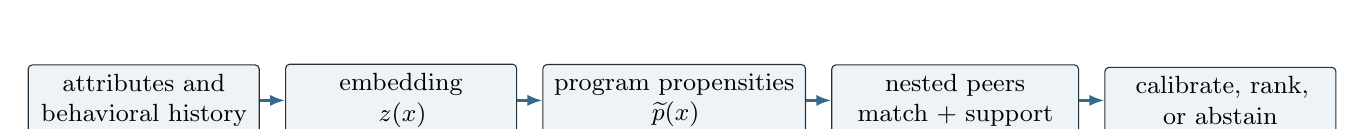
\begin{tikzpicture}[
  node distance=3.2mm,
  box/.style={draw=ink,rounded corners=1.5pt,fill=pale,align=center,minimum height=6.8mm,text width=27mm,font=\small},
  arrow/.style={-{Latex[length=1.9mm]},thick,draw=blue}
]
\node[box] (history) {attributes and\\behavioral history};
\node[box,right=of history] (embed) {embedding\\$z(x)$};
\node[box,right=of embed,text width=31mm] (scores) {program propensities\\$\widetilde p(x)$};
\node[box,right=of scores,text width=29mm] (near) {nested peers\\match $+$ support};
\node[box,right=of near,text width=27mm] (decision) {calibrate, rank,\\or abstain};
\draw[arrow] (history)--(embed);
\draw[arrow] (embed)--(scores);
\draw[arrow] (scores)--(near);
\draw[arrow] (near)--(decision);
\end{tikzpicture}
\refstepcounter{figure}
\par\vspace{0.7em}
\parbox{.94\linewidth}{\small\textbf{Figure \thefigure.} The embedding supplies the predictive representation. The neighborhood supplies local evidence and a measure of its reliability.}
\end{center}

\section{Propensities and behavioral embeddings}

Let $x$ denote a customer and let $\cA=\{a_1,\ldots,a_K\}$ be a catalog of $K$ programs. Eligibility leaves the feasible set $\cA(x)\subseteq\cA$. For program $a$, define the true enrollment propensity
\[
 p_a(x)=\Pr(\text{$x$ enrolls in $a$})\in[0,1].
\]
The vector $p(x)=(p_{a_1}(x),\ldots,p_{a_K}(x))$ is the customer's true propensity row. For customers $x_1,\ldots,x_N$, stacking these rows gives the true propensity matrix $P\in[0,1]^{N\times K}$. A fitted model produces rows $\widetilde p(x_i)$ and the fitted matrix $\widetilde P$. The direct recommender chooses
\begin{equation}\label{eq:base}
 \widetilde a(x)\in\argmax_{a\in\cA(x)}\widetilde p_a(x).
\end{equation}

Behavior provides useful customer coordinates. Let $H\in\mathbb R^{N\times J}$ record the pre-decision activity of $N$ customers over $J$ items or events. A rank-$D$ factorization gives
\[
 H\approx U_D\Sigma_DV_D^\top,
 \qquad z(x_i)=(U_D\Sigma_D)_{i\cdot}\in\mathbb R^D.
\]
Here $(\cdot)_{i\cdot}$ selects matrix row $i$, $^\top$ denotes transpose, and $z(x_i)$ is customer $i$'s behavioral embedding. If $s(x)$ is a vector of ordinary customer attributes, a program model has the form
\begin{equation}\label{eq:model}
 \widetilde p_a(x)=f_a\bigl(s(x),z(x)\bigr).
\end{equation}
This transparent factorization follows the collaborative-filtering tradition \cite{koren}; richer sequential representations could be used instead \cite{sasrec,bert4rec}. What matters is whether nearby coordinates identify customers with similar future propensities or similar remaining model errors.

\section{Nested neighborhoods}

Let $x_1,\ldots,x_n$ be historical reference customers. Divide the available customer representation into $M$ ordered blocks. After the first $m$ blocks, let $d_m(x,x_i)$ be the cumulative distance from target $x$ to reference customer $x_i$. We require
\[
 d_{m+1}(x,x_i)\ge d_m(x,x_i).
\]
For a fixed radius $r\ge0$, define the level-$m$ neighborhood and its size by
\begin{equation}\label{eq:neighborhood}
 \cN_m(x;r)=\{i:d_m(x,x_i)\le r\},
 \qquad n_m=|\cN_m(x;r)|.
\end{equation}
Only nonempty neighborhoods are used.

\begin{proposition}[More detail leaves fewer peers]\label{prop:thin}
For $m=1,\ldots,M-1$,
\[
 \cN_{m+1}(x;r)\subseteq\cN_m(x;r),
 \qquad n_{m+1}\le n_m.
\]
\end{proposition}

\begin{proof}
If $d_{m+1}(x,x_i)\le r$, then $d_m(x,x_i)\le d_{m+1}(x,x_i)\le r$. Every later-level peer was therefore already an earlier-level peer.
\end{proof}

To measure the quality of the remaining match, let $g(x)=(g_a(x):a\in\cA)$ be any program-indexed target. Define
\begin{equation}\label{eq:mismatch}
 \varepsilon_m^g(x)=
 \max_{i\in\cN_m(x;r)}\|g(x_i)-g(x)\|_\infty,
 \qquad \|v\|_\infty=\max_a|v_a|.
\end{equation}
For direct peer averaging, take $g=p$. For residual correction, take
\[
 g=\rho,
 \qquad \rho(x)=p(x)-\widetilde p(x).
\]
Thus $\rho(x)$ is the error left by the base propensity model.

\begin{proposition}[Refinement improves worst-case local similarity]\label{prop:mismatch}
If $\cN_{m+1}(x;r)$ is nonempty, then
\[
 \varepsilon_{m+1}^g(x)\le\varepsilon_m^g(x).
\]
\end{proposition}

\begin{proof}
The later neighborhood is a subset of the earlier one by Proposition~\ref{prop:thin}. The maximum of the same nonnegative quantity cannot increase when points are removed.
\end{proof}

These propositions describe the basic tension. Adding detail cannot worsen the worst match among the peers who remain, but it cannot add support. Propensity rows themselves provide a convenient geometry, for example
\[
 d_p(x,x_i)=\|\widetilde p(x)-\widetilde p(x_i)\|_\infty.
\]
A leave-one-program-out distance can omit coordinate $a$ when calibrating program $a$, although the experiments find that the omitted coordinate often contains useful retrieval information.

\section{The refinement frontier}

For peer $i$ and eligible program $a$, let $Y_{ia}\in[0,B]$ be a bounded calibration outcome with $\E[Y_{ia}\mid x_i]=p_a(x_i)$. Binary enrollment has $B=1$. Reference predictions must be out of fold or produced by a separately fitted model. At level $m$, correct the target score with the peers' mean residual:
\begin{equation}\label{eq:residual}
 \widehat p_{a,m}(x)=\widetilde p_a(x)
 +\frac{1}{n_m}\sum_{i\in\cN_m(x;r)}
 \bigl(Y_{ia}-\widetilde p_a(x_i)\bigr),
 \qquad
 \widehat a_m\in\argmax_{a\in\cA(x)}\widehat p_{a,m}(x).
\end{equation}
Clipping $\widehat p_{a,m}(x)$ to $[0,1]$ is optional. Let $a^*$ be a true best eligible program and let $K_x=|\cA(x)|$.

\begin{theorem}[Residual refinement frontier]\label{thm:frontier}
Suppose that, conditional on the customer profiles, $\{Y_{ia}:i=1,\ldots,n\}$ are independent for each $a$, and the neighborhoods are fixed from information independent of these outcomes. For a prespecified nonempty level $m$ and $\alpha\in(0,1)$, with probability at least $1-\alpha$,
\[
 p_{a^*}(x)-p_{\widehat a_m}(x)
 \le 2b_m(x),
 \qquad
 b_m(x)=\varepsilon_m^\rho(x)
 +B\sqrt{\frac{\log(2K_x/\alpha)}{2n_m}}.
\]
If the same calibration outcomes select one of $M$ levels, replace $K_x$ by $K_xM$.
\end{theorem}

\begin{proof}
Let $\bar\rho_{a,m}=n_m^{-1}\sum_{i\in\cN_m}\rho_a(x_i)$. The conditional mean of \eqref{eq:residual} is $\widetilde p_a(x)+\bar\rho_{a,m}$, and
\[
 |\bar\rho_{a,m}-\rho_a(x)|\le\varepsilon_m^\rho(x).
\]
Hoeffding's inequality and a union bound over the $K_x$ programs show that, simultaneously in $a$,
\[
 |\widehat p_{a,m}(x)-p_a(x)|\le b_m(x).
\]
Because $\widehat a_m$ maximizes the fitted values,
\[
 p_{a^*}(x)-p_{\widehat a_m}(x)
 \le[p_{a^*}-\widehat p_{a^*,m}]
 +[\widehat p_{\widehat a_m,m}-p_{\widehat a_m}]
 \le2b_m(x).
\]
A second union bound over the $M$ levels proves the adaptive statement.
\end{proof}

The bound has an intuitive form. The mismatch $\varepsilon_m^\rho$ decreases with refinement, while the sampling term grows as $n_m$ falls. Let $\widehat\varepsilon_m^\rho(x)$ be a validation estimate or upper-confidence estimate of the unknown mismatch. An estimated frontier chooses
\begin{equation}\label{eq:rule}
 \widehat m(x)\in\argmin_m
 \left\{
 \widehat\varepsilon_m^\rho(x)
 +B\sqrt{\frac{\log(2K_xM/\alpha)}{2n_m}}
 \right\}.
\end{equation}
The best level is not the most detailed one. It is the level at which a closer match is still worth the support it costs.

\subsection{An operational version}

The true target residual is unknown at recommendation time. Let $\widehat\rho(x)$ be a residual model trained separately from the target and reference outcomes. Write
\[
 R_i=Y_i-\widetilde p(x_i),
 \qquad
 c_m(x)=\lambda_m\frac{1}{n_m}\sum_{i\in\cN_m(x;r)}R_i,
 \qquad \lambda_m\in[0,1].
\]
Include level $m=0$ with $c_0(x)=0$. Define two observable discrepancies:
\begin{align*}
 D_m^{\rm mean}(x)&=\|\widehat\rho(x)-c_m(x)\|_\infty,\\
 D_m^{\rm max}(x)&=\lambda_m\max_{i\in\cN_m}
 \|\widehat\rho(x)-R_i\|_\infty
 +(1-\lambda_m)\|\widehat\rho(x)\|_\infty.
\end{align*}
Convexity gives $D_m^{\rm mean}\le D_m^{\rm max}$.

\begin{corollary}[Operational peer-mean frontier]\label{cor:operational}
Suppose an independently constructed simultaneous band satisfies
\[
 \Pr\{\|\rho(x)-\widehat\rho(x)\|_\infty\le\eta(x)\}\ge1-\delta.
\]
Choose $\widehat m(x)$ by minimizing either observable discrepancy, including level zero, without using $p(x)$. Then, with probability at least $1-\delta$,
\[
 \|p(x)-[\widetilde p(x)+c_{\widehat m}(x)]\|_\infty
 \le\eta(x)+D_{\widehat m}^{\rm mean}(x)
 \le\eta(x)+D_{\widehat m}^{\rm max}(x),
\]
and the selected program's propensity regret is at most twice the corresponding right-hand side.
\end{corollary}

\begin{proof}
Use the decomposition
\[
 \rho(x)-c_{\widehat m}(x)
 =[\rho(x)-\widehat\rho(x)]+[\widehat\rho(x)-c_{\widehat m}(x)]
\]
and apply the triangle inequality. Convexity gives the second inequality. The two-error argument in Theorem~\ref{thm:frontier} gives the regret result.
\end{proof}

This is a latent-propensity guarantee only when the band covers $\rho(x)$. Ordinary split conformal prediction instead gives a marginal statement about a future realized outcome. If the complete neighborhood algorithm is frozen before an independent calibration split, let $\widehat p^{\rm op}(x)$ denote its final score vector and define
\[
 S_i=\|Y_i-\widehat p^{\rm op}(x_i)\|_\infty,
\]
then the corrected split-conformal quantile $q_{1-\alpha}$ satisfies
\begin{equation}\label{eq:conformal}
 \Pr\{\|Y-\widehat p^{\rm op}(X)\|_\infty\le q_{1-\alpha}\}\ge1-\alpha
\end{equation}
under exchangeability \cite{shafer}. Realized-outcome regret is at most $2q_{1-\alpha}$ on this event. This is marginal coverage, not pointwise coverage of the conditional mean.

\begin{remark}[Known propensity coordinates]\label{rem:known}
If domain knowledge fixes $p_a(x)$ at zero or one, then its residual is known exactly and its uncertainty radius can be set to zero. Only the unknown coordinates need a residual band.
\end{remark}

\begin{corollary}[A confident recommendation]\label{cor:margin}
Assume $K_x\ge2$. Let the corrected winner have empirical lead
\[
 \Delta_m(x)=\widehat p_{\widehat a_m,m}(x)
 -\max_{a\in\cA(x),\,a\ne\widehat a_m}\widehat p_{a,m}(x).
\]
On the event in Theorem~\ref{thm:frontier}, if $\Delta_m(x)>2b_m(x)$, then $\widehat a_m$ is the unique true best program.
\end{corollary}

\begin{proof}
Every true propensity is within $b_m$ of its estimate. A fitted lead larger than $2b_m$ stays positive even after both scores move by their largest permitted errors.
\end{proof}

Shrinkage replaces the raw correction by $\lambda c_m$. Its uniform error is at most
\[
 (1-\lambda)\|\rho(x)\|_\infty
 +\lambda\varepsilon_m^\rho(x)
 +\lambda B\sqrt{\frac{\log(2K_x/\alpha)}{2n_m}}.
\]
Validation can choose $\lambda$. In practice, rerank only when local evidence clears the relevant margin bound; otherwise retain the base choice or flag low confidence.

\section{How the system runs}

The mathematics maps to a short operating loop:
\begin{enumerate}[label=\textbf{\arabic*.},itemsep=.35ex]
\item \textbf{Filter eligibility.} Form $\cA(x)$ before scoring.
\item \textbf{Represent the customer.} Learn $z(x)$ from pre-decision history and combine it with $s(x)$.
\item \textbf{Score the catalog.} Fit $\widetilde p_a(x)=f_a(s(x),z(x))$ and create out-of-fold reference rows.
\item \textbf{Retrieve nested peers.} Add declared feature blocks so $\cN_1\supseteq\cdots\supseteq\cN_M$.
\item \textbf{Balance match and support.} Record mismatch, $n_m$, and the frontier objective in \eqref{eq:rule}; level zero keeps the base model.
\item \textbf{Decide.} Apply a supported residual correction, compare the top margin with its bound, and recommend, retain the base ranking, or abstain.
\end{enumerate}
This retrieve-and-rank structure is common in large recommender systems \cite{covington}. Here the neighborhood and certificate decide whether local evidence is strong enough to modify the score.

\section{Evidence from KuaiRec}

KuaiRec contains nearly complete viewing records for 1,411 users and 3,327 videos \cite{gao}. We use the twelve largest video categories as program analogues. A user's category propensity is the fraction of videos watched to completion. For each user, the first 60\% of interactions form the observable history and the last 40\% form future targets. In each repeated split, 60\% of users estimate the models and out-of-fold residuals, 25\% tune neighborhood choices, and 15\% are untouched test users. A 32-coordinate SVD embedding is fit from estimation histories only.

\begin{center}
\refstepcounter{table}
\parbox{.94\linewidth}{\small\textbf{Table \thetable.} Mean chronological test performance over ten splits. Lower RMSE and regret are better; higher hit rate is better. Panel B uses ten fresh splits after the propensity-neighborhood rule was frozen.}
\vspace{.25em}

\small
\begin{tabular}{lccc}
\toprule
Method & RMSE & Top-1 regret & Hit rate \\
\midrule
\multicolumn{4}{l}{\emph{Panel A: behavioral representation}}\\
Static customer features & 0.126761 & 0.041357 & 34.46\%\\
Static $+$ behavioral embedding & 0.086310 & 0.038726 & 37.04\%\\
Embedding-space shared neighbors & 0.085960 & \textbf{0.038530} & \textbf{37.09\%}\\
Embedding-space program-specific neighbors & \textbf{0.085564} & 0.039276 & 36.48\%\\
\midrule
\multicolumn{4}{l}{\emph{Panel B: propensity-space confirmation}}\\
Static $+$ behavioral embedding & 0.083850 & \textbf{0.036119} & \textbf{39.30\%}\\
Full-row propensity neighbors & \textbf{0.083498} & 0.036931 & 38.83\%\\
Leave-one-program-out neighbors & 0.083833 & 0.037950 & 37.51\%\\
\bottomrule
\end{tabular}
\end{center}

The embedding is the main result. Relative to static features, it lowers RMSE by 31.9\%, lowers regret by 6.4\%, and raises hit rate by 2.58 percentage points. RMSE improves in all ten splits, regret in eight, and hit rate in nine. The learned representation therefore captures useful future behavior before any local correction is applied.

Neighborhoods have a smaller role. Full-row propensity neighborhoods improve RMSE in nine of ten fresh splits, but their mean regret is 2.2\% worse than direct embedding-based ranking. Leave-one-program-out matching is weaker. Better calibration does not necessarily identify a better winner.

A separate leakage-free operational experiment uses disjoint groups to fit the base model, fit $\widehat\rho$, supply reference residuals, calibrate conformal scores, and evaluate the frozen rule. It aggregates 4,280 held-out-user evaluations.

\begin{center}
\refstepcounter{table}
\parbox{.94\linewidth}{\small\textbf{Table \thetable.} Operational fixed-radius diagnostic over twenty disjoint splits. Neighborhood use is the fraction of test users receiving a peer correction.}
\vspace{.25em}

\small
\begin{tabular}{lrrrr}
\toprule
Method & RMSE & Regret & Hit rate & Use \\
\midrule
Base model & 0.110439 & 0.019361 & 49.18\% & 0.00\%\\
Theorem-faithful max frontier & 0.110438 & 0.019361 & 49.18\% & 0.09\%\\
Operational peer-mean frontier & \textbf{0.110129} & \textbf{0.019257} & \textbf{49.35\%} & 63.36\%\\
Legacy score-space proxy & 0.110318 & 0.019429 & 49.00\% & 100.00\%\\
\bottomrule
\end{tabular}
\end{center}

The peer-mean frontier lowers RMSE by 0.000310; its descriptive paired 95\% interval is $[-0.000560,-0.000060]$. Regret and hit-rate intervals include zero. End-to-end split conformal calibration attains 90.9\% coverage at nominal 90\%, but its mean regret bound, 0.5053, is slightly wider than the base benchmark, 0.5018. No top-two margin is wide enough to certify an individual winner. The experiments therefore support a modest calibration benefit, not an additional ranking gain.

The earlier fixed-radius pilot also displays the geometric mechanism: later blocks rapidly remove peers, and performance worsens when refinement outruns support. The support-aware rule avoids the deepest level. This is what the frontier is designed to control.

\section{Interpretation}

The practical recommendation is straightforward: use behavioral embeddings in the propensity model and rank its eligible outputs directly. Keep the neighborhood layer when local calibration, diagnostics, or confidence information is valuable. The theorem tells the system when a correction has enough support; it does not assume that useful local residual structure exists in every dataset.

The target also matters. Enrollment propensity is not the same as incremental enrollment, energy savings, or economic value. If a causal effect is identified under an appropriate assignment and policy-evaluation design, that effect can replace $p_a(x)$ in the workflow \cite{dudik}. Recent energy studies show the value of targeting heterogeneous conservation and retrofit effects \cite{knittel,christensen}. The present analysis is narrower: it studies enrollment propensity and the reliability of local correction.

The resulting story has three parts. Behavioral history supplies a useful geometry. Nested neighborhoods make local evidence more specific while spending peer support. The refinement frontier prices that trade and supports a calibrated recommendation, a retained base ranking, or an honest decision to abstain.

\begin{thebibliography}{99}\small\setlength{\itemsep}{0pt}\setlength{\parskip}{0pt}

\bibitem{koren}
Y. Koren, R. Bell, and C. Volinsky, ``Matrix factorization techniques for recommender systems,'' \emph{Computer}, 42(8):30--37, 2009.

\bibitem{sasrec}
W.-C. Kang and J. McAuley, ``Self-attentive sequential recommendation,'' in \emph{Proc. ICDM}, pp. 197--206, 2018.

\bibitem{bert4rec}
F. Sun et al., ``BERT4Rec: Sequential recommendation with bidirectional encoder representations from Transformer,'' in \emph{Proc. CIKM}, pp. 1441--1450, 2019.

\bibitem{shafer}
G. Shafer and V. Vovk, ``A tutorial on conformal prediction,'' \emph{JMLR}, 9:371--421, 2008.

\bibitem{covington}
P. Covington, J. Adams, and E. Sargin, ``Deep neural networks for YouTube recommendations,'' in \emph{Proc. RecSys}, pp. 191--198, 2016.

\bibitem{gao}
C. Gao et al., ``KuaiRec: A fully-observed dataset and insights for evaluating recommender systems,'' in \emph{Proc. CIKM}, pp. 540--550, 2022.

\bibitem{dudik}
M. Dud\'{i}k, J. Langford, and L. Li, ``Doubly robust policy evaluation and learning,'' in \emph{Proc. ICML}, pp. 1097--1104, 2011.

\bibitem{knittel}
C. R. Knittel and S. Stolper, ``Using machine learning to target treatment: The case of household energy use,'' \emph{Economic Journal}, 135(672):2377--2401, 2025.

\bibitem{christensen}
P. Christensen et al., ``Energy efficiency can deliver for climate policy: Evidence from machine learning-based targeting,'' \emph{Journal of Public Economics}, 234:105098, 2024.

\end{thebibliography}

\end{document}
